\documentclass[12pt]{article}
\usepackage{amsmath}
\usepackage{amsfonts}
\usepackage{graphicx}
\usepackage{hyperref}
\usepackage [a4paper, left=2.5cm, right=2.5cm] {geometry}
\usepackage{float}
\usepackage{indentfirst}
\usepackage{longtable}
\usepackage{verbatim}

\geometry{a4paper}


% Domain assumption reliable connection

\begin{titlepage}

\title{Requirement Analysis and Specification Document (RASD)}
\author{Group Name: Davide Rodler, Stefano Riva \\ Version: 1.0 \\ Date: [Submission Date]}
\date{}

\end{titlepage}

%Andrebbe messo il titolo in una pagina e la tableofcontents in un'altra

\begin{document}

\maketitle

\tableofcontents

\section{Introduction}

\subsection{Purpose}
The \textbf{Students\&Companies (S\&C)} platform is designed to address the challenges of matching university students with companies offering internships. These challenges include difficulties for students in identifying suitable internships aligned with their skills and career aspirations, and for companies in efficiently finding qualified candidates for their positions.

The platform enables students to search for internships, receive personalized recommendations, and manage their applications. For companies, it provides tools to advertise internships, review candidate CVs, and manage the interview and selection process. By leveraging recommendation mechanisms and supporting the selection process, the platform ensures an efficient and mutually beneficial experience for both students and companies.

\subsubsection{Goals}
\begin{itemize}
    \item \textbf{[G1]} The platform should facilitate the matchmaking process between university students and companies offering internships.
    \item \textbf{[G2]} The platform should enable companies to search for and evaluate student profiles that meet their internship requirements.
    \item \textbf{[G3]} The platform should allow students to search for internships aligned with their skills, experiences, and career goals.
    \item \textbf{[G4]} The platform should support companies in managing the internship selection process, including interviews.
\end{itemize}

\subsection{Scope}
The S\&C platform is intended for three main stakeholders: students, companies. 
\begin{itemize}
    \item \textbf{Students}: Can create and upload CVs, search for internships, receive recommendations, and manage their application and interview processes.
    \item \textbf{Companies}: Can advertise internship opportunities, review student applications, conduct interviews, and finalize selections.
\end{itemize}
The platform is scalable and can accommodate a wide range of internships and users, including undergraduate and postgraduate students, small businesses, and large corporations.
The platform also collects feedback from both students and companies, which is used to improve the recommendation mechanisms and provide insights into the effectiveness of internships.

\subsubsection{World Phenomena}
\begin{itemize}
    \item \textbf{[WP1]} Students prepare their CVs
    \item \textbf{[WP2]} Students upload their CVs.
    \item \textbf{[WP3]} Companies define internship projects and specify their terms.
\end{itemize}

\subsubsection{Shared Phenomena}
\begin{itemize}
    \item \textbf{[SP1]} Students search for internships on the platform. \textbf{[WC]}
    \item \textbf{[SP2]} Companies advertise internships on the platform. \textbf{[WC]}
    \item \textbf{[SP3]} The system informs students about internships that match their profiles. \textbf{[MC]}
    \item \textbf{[SP4]} The system informs companies of student profiles matching their internship requirements. \textbf{[MC]}
    \item \textbf{[SP5]} The system facilitates communication between students and companies. \textbf{[MC]}
    \item \textbf{[SP6]} The platform supports the scheduling and management of interviews. \textbf{[MC]}
    \item \textbf{[SP7]} The system notifies companies when students matching their requirements become available. \textbf{[MC]}
    \item \textbf{[SP8]} When suitable recommendations are identified and accepted by both parties, a contact is established. \textbf{[MC]}
    \item \textbf{[SP9]} The company selects a student from the list of students compatible with the internship offer. \textbf{[WC]}
    \item \textbf{[SP10]} Users provide feedback. \textbf{[WC]}
    \item \textbf{[SP11]} Companies advertise their internships on the platform. \textbf{[WC]}
    \item \textbf{[SP12]} Students upload their CVs to the platform. \textbf{[WC]}
    \item \textbf{[SP13]} Companies conduct interviews to assess candidates for internships. \textbf{[WC]}
\end{itemize}


\subsection{Definitions, Acronyms, and Abbreviations}
\subsubsection{Definitions}
\begin{itemize}
    \item \textbf{CV Curriculum Vitae}: Document detailing a student's skills, experiences, and educational background.
    \item \textbf{Internship}: Temporary professional experience provided by a company to a student, typically aligned with their field of study.
    \item \textbf{Recommendation System}: Mechanism for suggesting matches between students and companies based on complex mechanism, like keyword searching and statistical analysis.
\end{itemize}

\subsubsection{Acronyms}
\begin{itemize}
    \item \textbf{S\&C}: Students\&Companies.
    \item \textbf{CV}: Curriculum Vitae.
    \item \textbf{UI}: User Interface.
\end{itemize}

\subsubsection{Abbreviations}
\begin{itemize}
    \item \textbf{G*}: Goals outlined in the Purpose section.
    \item \textbf{WP*}: World phenomena describing activities by individual stakeholders.
    \item \textbf{SP*}: Shared phenomena describing system-mediated interactions.
    \item \textbf{R*}: Functional requirements.
    \item \textbf{UC*}: Use cases.
\end{itemize}

\subsection{Revision History}
\begin{itemize}
    \item Version 1.0 () %TODO: Inserire la data di completamento
\end{itemize}

\subsection{Reference Documents}
\begin{itemize}
    \item Project Specification Document provided by the course professors.
    \item Course slide on WeBeep
    \item IEEE Standards for Requirements Specifications.
\end{itemize}

\subsection{Document Structure}
This document is structured as follows:
\begin{itemize}
    \item \textbf{Section 1 - Introduction}: Describes the project's purpose, goals, scope, and related definitions.
    \item \textbf{Section 2 - Overall Description}: Provides an overview of the system, including scenarios, domain models, and functionalities.
    \item \textbf{Section 3 - Specific Requirements}: Provides details on the functional and non-functional requirements of the system.
    \item \textbf{Section 4 - Formal Analysis}: Includes Alloy-based formalization of world phenomena.
    \item \textbf{Section 5 - Effort Spent}: Summarizes the effort distribution among team members.
    \item \textbf{References}: Lists reference documents and resources used.
\end{itemize}

\newpage

\section{Overall Description}

\subsection{Product Perspective}

\subsubsection{Scenarios}

\textbf{A Company Advertises an Internship} \\
Company A, which is looking to hire interns, logs into the Students\&Companies (S\&C) platform using its credentials. Once logged in, the company accesses the section to "Create a New Internship." Here, Company A carefully fills out a form detailing the internship project, including the application domain, tasks to be performed, and any relevant technologies that will be used. The company also specifies the terms of the internship, such as whether it is paid, and outlines additional benefits like training, mentorship, or certifications. After reviewing the information, Company A publishes the internship, making it visible to all students on the platform who may be interested.

\vspace{0.5cm}

\textbf{A Student Publishes Their CV} \\
Student B, who is seeking an internship, begins by preparing a CV that highlights their skills, experiences, and academic achievements. If they don’t already have a CV, they create one specifically for the platform. After ensuring their CV is complete and accurate, Student B logs into the S\&C platform using their credentials. Once logged in, they navigate to the section for uploading a CV, submit the document, and make it available for companies to view. This step ensures that their profile is visible to potential employers on the platform.

\vspace{0.5cm}

\textbf{The Recommendation System Notifies a Student} \\
Student D, who has uploaded their CV to the platform, receives a notification from the S\&C recommendation system. The system, analyzing the student's CV and preferences, identifies that a new internship offered by Company B matches their profile. The notification contains details about the internship, including the project, tasks, and terms. Student D reviews the information and decides to apply for the internship, using the platform to submit their application.

\vspace{0.5cm}

\textbf{The Recommendation System Notifies a Company} \\
Company E, which has posted multiple internships on the S\&C platform, receives a notification from the recommendation system. The system identifies that Student F, who recently uploaded their CV, matches the criteria set for one of the internships. The company reviews the student's profile and decides to contact them through the platform to discuss potential collaboration.

\vspace{0.5cm}

\textbf{A Contact is Established Between a Student and a Company} \\
Student G and Company H, after being matched through the recommendation system, both express interest in proceeding with the opportunity. The S\&C platform facilitates a formal contact between the two parties, enabling them to communicate directly. This marks the beginning of the selection process.

\vspace{0.5cm}

\textbf{A Company Conducts an Interview} \\
Company I, having reviewed Student J’s CV and established contact through the platform, schedules an interview to evaluate their suitability for the internship. The interview is conducted through the S\&C platform and may include a structured questionnaire prepared by the company. During the session, Student J answers questions about their experiences, skills, and motivations. The company uses the responses to assess whether the student fits the requirements of the internship project.

\vspace{0.5cm}

\textbf{A Student Applies Proactively to an Internship} \\
Student K, who prefers to take initiative, logs into the S\&C platform to browse the list of internships. After filtering opportunities based on their skills and interests, they apply to an internship offered by Company L. The application process involves uploading their CV, attaching relevant documents if necessary, and submitting the application directly through the platform. Student K eagerly awaits a response from the company.

\vspace{0.5cm}

\textbf{A Company Evaluates Candidates} \\
Company M, after receiving multiple applications for an internship, reviews the submitted CVs through the S\&C platform. Using filtering tools provided by the platform, the company shortlists candidates whose skills and experiences match the requirements of the internship. They then proceed to schedule interviews with the shortlisted students.

\vspace{0.5cm}

\textbf{A Student Joins an Internship} \\
After successfully completing the interview process with Company N, Student O receives an offer for the internship through the platform. The platform notifies the student of their acceptance and provides details about the next steps. Student O confirms their acceptance, and the internship officially begins.


\newpage

\subsubsection{Domain Class Diagram}

\begin{figure}[H]
    \centering
    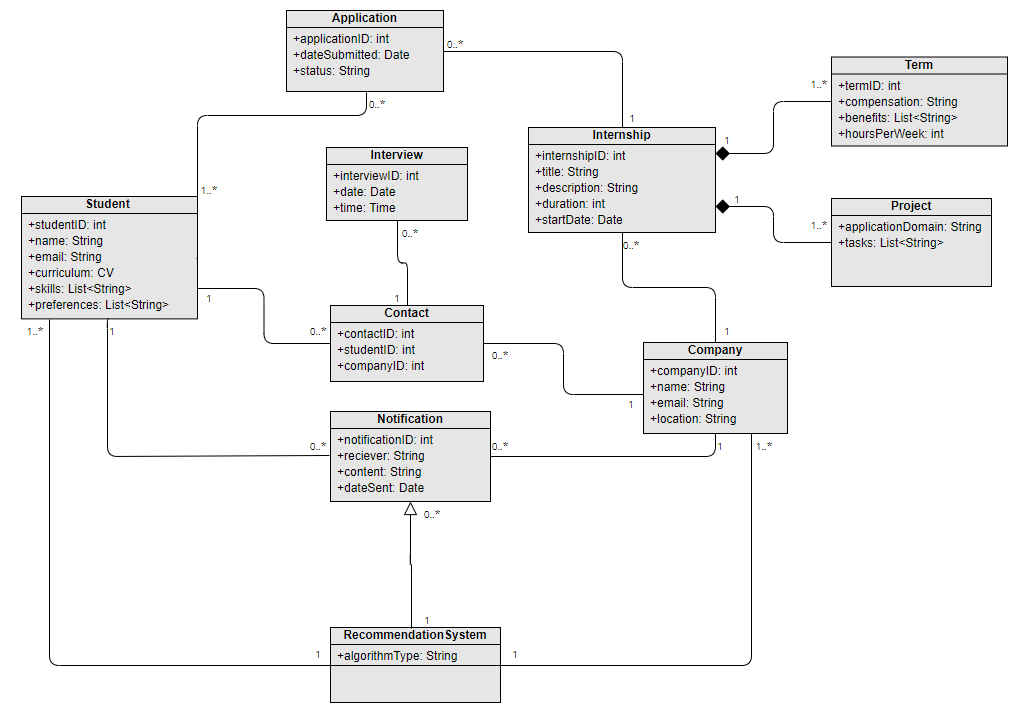
\includegraphics[scale=0.62]{rasd_diagrams/Class-Diagram.png}
    \caption{\scriptsize \textbf{Domain Class Diagram of the Students\&Companies (S\&C) Platform}}
    \label{fig:domain_class_diagram}
\end{figure}

\vspace{3cm}

In Figure~\ref{fig:domain_class_diagram}, the domain class diagram models the key entities and their relationships in the \textbf{Students\&Companies (S\&C)} platform. This platform facilitates the internship matching process by connecting students and companies, managing their interactions from application to selection. The diagram captures the roles of students, companies, and the system components in achieving these objectives.
The \textbf{Student} class represents users seeking internships. Each student can create multiple \textbf{Applications} for different internships offered by companies. The \textbf{Company} class represents organizations advertising internships, which are defined through the composition of \textbf{Project} and \textbf{Term} components. These define the domain, tasks, and conditions of the internship, such as compensation and benefits.
The \textbf{RecommendationSystem} class facilitates matching by analyzing student profiles and internship requirements. Notifications are sent to students and companies to inform them about matches or updates via the \textbf{Notification} class. Once a recommendation is accepted, a \textbf{Contact} is established between the student and the company, which leads to the \textbf{Interview} process for final evaluation.
The \textbf{Application} class tracks the submission and status of internship applications, while the \textbf{Interview} class manages scheduled sessions between students and companies.

\paragraph{Details of the Classes and Relationships}
\begin{itemize}
    \item \textbf{Student}: Represents users looking for internships. Each student has a unique ID, name, email, CV, and a set of skills and preferences. Students can submit applications, receive notifications, and interact with the recommendation system.
    \item \textbf{Company}: Represents organizations offering internships. Companies can advertise internships, receive notifications about suitable candidates, and interact with students after establishing a contact.
    \item \textbf{Internship}: Represents internship opportunities advertised by companies. Each internship is defined by a project and its associated terms.
    \item \textbf{Project}: Describes the domain, tasks, and technologies related to an internship.
    \item \textbf{Term}: Defines the terms and conditions of the internship, including compensation and benefits.
    \item \textbf{RecommendationSystem}: Facilitates the matching process by generating recommendations for students and companies.
    \item \textbf{Notification}: Represents updates or messages sent to students and companies about matches or system events.
    \item \textbf{Application}: Tracks each student's application to internships, including its status and submission date.
    \item \textbf{Contact}: Represents the established link between a student and a company after a recommendation is accepted.
    \item \textbf{Interview}: Manages the scheduling and details of interviews between students and companies.
\end{itemize}
The diagram represents the key functionality of the platform, ensuring all interactions and relationships between students, companies, and the system components are captured.

\newpage

\subsubsection{ State Diagrams}

In this subsection, a discussion is provided regarding the state charts diagram for the internship application process. This diagram is essential for understanding the various states and transitions involved in managing the life cycle of an internship application.

\vspace{2cm}
\textbf{\footnotesize{Internship Application Management}} 
\vspace{0.1cm}

\begin{figure}[H]
    \centering
    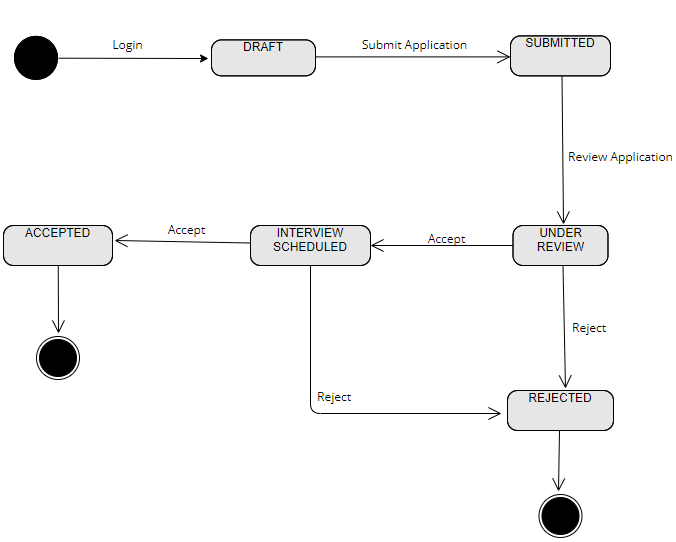
\includegraphics[scale=0.8]{rasd_diagrams/InternshipStateDiagram.png}
    \caption{\textbf{State Diagram for Internship Application Process}}
    \label{fig:internship_state_chart}
\end{figure}

In this state charts diagram, the different states and transitions involved in the internship application process are represented. The process begins when a student logs into the platform, initiating the state of \textbf{Draft}, where they can prepare their application. The \textbf{Submitted} state is reached after the student submits their application.

Once submitted, the application moves to the \textbf{Under Review} state, where the company evaluates it. At this stage, two possible transitions exist: if the company rejects the application, it moves to the \textbf{Rejected} state; if the application meets the requirements, it transitions to the \textbf{Interview Scheduled} state.

During the \textbf{Interview Scheduled} state, the student participates in an interview, after which two outcomes are possible. If the interview is successful, the application transitions to the \textbf{Accepted} state, signifying that the student has secured the internship. Conversely, if the company decides not to proceed, the application transitions to the \textbf{Rejected} state.

The process ends when the application reaches either the \textbf{Accepted} or \textbf{Rejected} state, with both being terminal states in the diagram.


\newpage

\subsection{Product Functions}

\subsubsection{Sign-up and Log-in}
This function is available to all users who want to subscribe to the platform. When a new user opens the platform, they can press the button 'Sign-up'. The system then redirects the user to the registration page, where they can create an account by providing their email, username, and password. Once the account is created, the user can log in to the platform with their credentials to access the system functionalities. %Come gestiamo la differenza tra studenti e companies?

\subsubsection{Internship Management by Companies}
This function allows companies to manage internship opportunities. After logging in, a company can create an internship by filling out a form specifying the internship’s application domain, tasks to be performed, technologies (if applicable), and terms offered (e.g., paid internships, training, mentorship). Companies can also edit or delete their published internships based on their evolving needs. Furthermore, companies are notified by the system when students matching their criteria upload new CVs to the platform.

\subsubsection{CV Management by Students}
Students can create and upload their CVs using this function. Once logged into the platform, students are directed to a section where they can fill in their skills, experiences, and educational background to generate a CV. Students can update or replace their CVs whenever necessary to reflect their most recent achievements. The platform ensures that uploaded CVs are visible to companies searching for suitable candidates. %Avevamo messo come domain assumption che lo studente creava il CV fuori dalla piattaforma

\subsubsection{Search and Application for Internships}
This function allows students to browse and search for internships posted by companies. Students can filter internships based on domains, tasks, technologies, or terms. Once a student identifies a suitable internship, they can submit their application by attaching their CV and any additional required information. This application is stored in the platform and made available to the corresponding company for review.

\subsubsection{Recommendation System}
The platform integrates a recommendation system to streamline the internship matching process. For students, the system analyzes their uploaded CVs and preferences to suggest internships that align with their skills and career aspirations. Similarly, for companies, the system suggests students whose profiles meet their specified requirements. These recommendations are displayed as notifications, allowing both parties to evaluate and act on potential matches efficiently.

\subsubsection{Interview Scheduling and Management}
This function supports the interview process between students and companies. Once a company shortlists a student’s application, they can use the platform to schedule an interview. The system provides tools for managing the interview, such as setting dates and sharing structured questionnaires. Notifications about scheduled interviews are sent to both students and companies, ensuring effective communication and coordination.

\subsubsection{Application Status Tracking}
Students can track the status of their internship applications through this function. Applications transition between states such as \textit{Submitted}, \textit{Under Review}, \textit{Interview Scheduled}, \textit{Accepted}, and \textit{Rejected}. These status updates are visible on the student’s dashboard, providing real-time insights into their application progress. %Secondo me esce troppo dalla specifica, soprattutto quando proponi 4 stati della domanda, lì si entra un po' troppo nella fase di design

\subsubsection{Internship Acceptance and Finalization}
Once the interview process concludes, companies can accept or reject applications. Accepted applications transition to a finalized state, and the student receives an offer notification. This function ensures that both parties have clear and structured communication regarding the outcome, marking the official start of the internship.

\newpage

\subsection{2.3 User Characteristics}

There are two main types of users that interact with the platform: students and companies.

\subsubsection{Student}
A student is able to register and log in to the platform. Students can search for internships, upload their CVs, and participate in the recommendation and selection process. They can also be notified by the system when internships matching their profiles become available.

\subsubsection{Company}
A company is a user that advertises internships on the platform. Companies can create internship offers, review student applications, and manage the selection process, including scheduling interviews. They also receive notifications when suitable candidates are identified by the system.



\newpage

\section{Specific Requirements}

\subsection{External Interface Requirements}

\subsubsection{User Interfaces}

\subsubsection{Hardware Interfaces}

\subsubsection{Communication Interfaces}

\subsection{Functional Requirements}

    \textbf{Log in and Sign up}
        \begin{itemize}
            \item \textbf{[R1]} The system allows users to register to the platform.
            \item \textbf{[R2]} The system allows users to login to the platform through their credentials.
        \end{itemize}
    \textbf{Functionalities}
        \begin{itemize}
            \item \textbf{[R3]} The system permits students to upload their CVs.
            \item \textbf{[R4]} The system permits students to modify their CVs.
            \item \textbf{[R5]} The system permits students to proactively search for internships.
            \item \textbf{[R6]} The system permits companies to publish their internship proposal.
            \item \textbf{[R7]} The system permits companies to modify their internship proposal.
            \item \textbf{[R8]} The system permits companies to delete their internship proposal.
        \end{itemize}
    \textbf{Encapsulation}
        \begin{itemize}
            \item \textbf{[R9]} The system shows students only the internship proposals.
            \item \textbf{[R10]} The system shows companies only students CVs.
        \end{itemize}
    \textbf{Recommendation System}
        \begin{itemize}
            \item \textbf{[R11]} If a student with a CV which is compatible with the company requests is available then the system notify the company about this student.
            \item \textbf{[R12]} If an internship which matches the interests of the student is available then the system notifies the student about this internship.
        \end{itemize}
    \textbf{Interaction between students and companies}
        \begin{itemize}
            \item \textbf{[R13]} The system permits the student to submit their application to an internship they are interested in.
            \item \textbf{[R14]} The system permits the companies to assess the students applications.
        \end{itemize}
    \textbf{Selection Process}
        \begin{itemize}
            \item \textbf{[R15]} If the user is interested, the system permits him to accept the recommendation.
            \item \textbf{[R16]} If both the company and the student accept the recommendation, the system puts them in contact.
            \item \textbf{[R17]} If the company and the student have been put in contact then the system starts the selection process.
            \item \textbf{[R18]} The system helps the company managing the interview.
            \item \textbf{[R19]} If the interview went well (the company is satisfied with the answers provided by the student), the system finalize the selection.
        \end{itemize}
    \textbf{Feedback}
        \begin{itemize}
            \item \textbf{[R20]} The system collects the feedback from the users.
            \item \textbf{[R21]} The system uses collected feedback to feed statistical analysis applied during recommendation.
        \end{itemize}
    

\subsubsection{Use Case Diagram}
    \begin{figure}[H]
        \centering
        \hspace*{-1cm}
        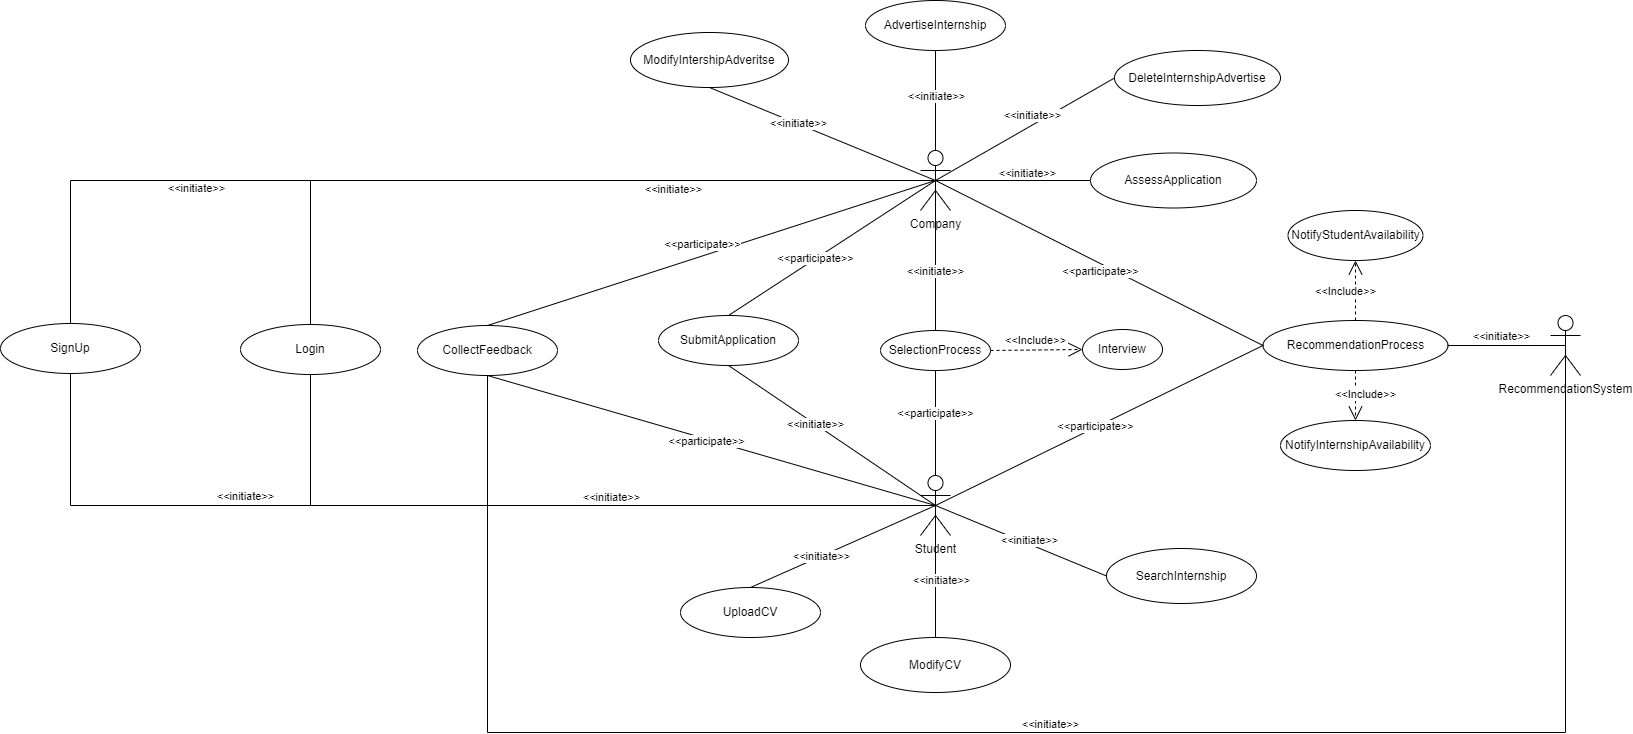
\includegraphics[scale = 0.3]{rasd_diagrams/UseCaseDiagram_v_1_4.png}
        \caption{\textbf{Use Case Diagram}}
        \label{fig:use_case_diagram}
    \end{figure}

    %Inserire descrizione

\subsubsection{Use Cases}
    \begin{itemize}
        \item \textbf{[UC1] - Sign-Up}
        \item \textbf{[UC2] - Log-in}
        \item \textbf{[UC3] - Upload CV}
        \item \textbf{[UC4] - Modify CV}
        \item \textbf{[UC5] - Advertise internship}
        \item \textbf{[UC6] - Modify internship advertise}
        \item \textbf{[UC7] - Delete internship advertise}
        \item \textbf{[UC8] - Search internships}
        \item \textbf{[UC9] - Recommendation process}
        \item \textbf{[UC10] - Submit application}
        \item \textbf{[UC11] - Assess application}
        \item \textbf{[UC12] - Collect feedback}
        \item \textbf{[UC13] - Selection process}
    \end{itemize}

\subsubsection{Sequence Diagrams}
    \textbf{[UC1] - Sign-Up}
    
        \begin{figure}[H]
            \centering
            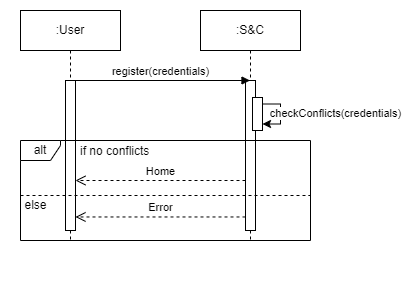
\includegraphics[scale = 0.7]{sequence_diagrams/SequenceDiagramSignUp_v_1_0.png}
            \caption{Sign-up}
            \label{fig:sign_up_sequence_diagram}
        \end{figure}
        
        \begin{center}
            \begin{longtable}{|l|p{0.75\linewidth}|}
                \hline
                \textbf{Name}
                & Sign-up \\
                \hline
                \textbf{Actors}
                & User (Student or Company) \\
                \hline
                \textbf{Entry Condition}
                & The user is not registered and connects to the site URL. \\
                \hline
                \textbf{Event Flow}
                & 1 - User compiles the registration form. \\
                & 2 - User sends the form to S\&C platform which checks the information provided. \\
                \hline
                \textbf{Exit Condition}
                & If there are no conflicts in the user's info (for example, username already used), the registration process terminates correctly, and the homepage is sent to the user. \\
                \hline
                \textbf{Exception}
                & The user is already registered. \\
                & Conflicts in the information sent by the user. \\
                \hline
            \end{longtable}
        \end{center}
        
    \newpage
    
    \textbf{[UC2] - Log-in}
    
        \begin{figure}[H]
            \centering
            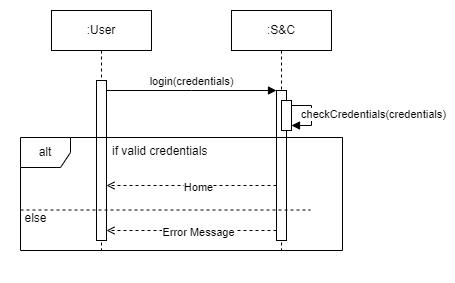
\includegraphics[scale = 0.7]{sequence_diagrams/SequenceDiagramLogin_v_1_0.png}
            \caption{Log-in}
            \label{fig:log_in_sequence_diagram}
        \end{figure}

        \begin{center}
            \begin{longtable}{|l|p{0.75\linewidth}|}
                \hline
                \textbf{Name}
                & Log-in \\
                \hline
                \textbf{Actors}
                & User (Student or Company) \\
                \hline
                \textbf{Entry Condition}
                & The user is registered but not logged in and tries to connect to the site URL. \\
                \hline
                \textbf{Event Flow}
                & 1 - User compiles the log-in form. \\
                & 2 - User sends the form to S\&C platform which checks the information provided. \\
                \hline
                \textbf{Exit Condition}
                & User's info are correct and the homepage is sent to the user. \\
                \hline
                \textbf{Exception}
                &  User's info don't match the ones stored in the database. \\
                \hline
            \end{longtable}
        \end{center}

    \newpage
    
    \textbf{[UC3] - Upload CV}
    
        \begin{figure}[H]
            \centering
            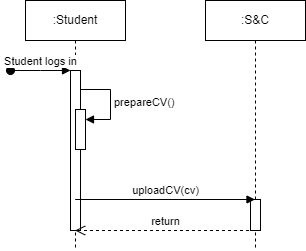
\includegraphics[scale = 0.7]{sequence_diagrams/SequenceDiagramUploadCV_v_1_1.png}
            \caption{Log-in}
            \label{fig:upload_cv_sequence_diagram}
        \end{figure}

        \begin{center}
            \begin{longtable}{|l|p{0.75\linewidth}|}
                \hline
                \textbf{Name}
                & Upload CV \\
                \hline
                \textbf{Actors}
                & Student \\
                \hline
                \textbf{Entry Condition}
                & Student does not have a CV associated to his profile and logs into the site. \\
                \hline
                \textbf{Event Flow}
                & 1 - Student prepares his CV writing his experiences and personal information.\\
                & 2 - Student upload his CV to the platform. \\
                \hline
                \textbf{Exit Condition}
                & Student's CV is correctly uploaded on the platform. \\
                \hline
                \textbf{Exception}
                &  No exception \\
                \hline
            \end{longtable}
        \end{center}

    \newpage
    
    \textbf{[UC4] - Modify CV}
    
        \begin{figure}[H]
            \centering
            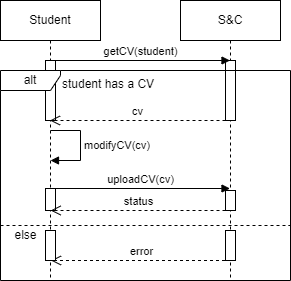
\includegraphics[scale = 0.7]{sequence_diagrams/SequenceDiagramModifyCV_v_1_0.png}
            \caption{Log-in}
            \label{fig:modify_cv_sequence_diagram}
        \end{figure}

        \begin{center}
            \begin{longtable}{|l|p{0.75\linewidth}|}
                \hline
                \textbf{Name}
                & Modify CV \\
                \hline
                \textbf{Actors}
                & Student \\
                \hline
                \textbf{Entry Condition}
                & Student wants to modify his CV. \\
                \hline
                \textbf{Event Flow}
                & 1 - Student opens his CV.\\
                & 2 - Student modifies his CV. \\
                & 3 - Student uploads his modified CV to the platform. \\
                \hline
                \textbf{Exit Condition}
                & Student's CV is correctly modified and uploaded on the platform. \\
                \hline
                \textbf{Exception}
                &  Student does not possess a CV. \\
                \hline
            \end{longtable}
        \end{center}

    \newpage
        
    \textbf{[UC5] - Advertise internship}
    
        \begin{figure}[H]
            \centering
            
\includegraphics[scale = 0.7]{sequence_diagrams/SequenceDiagramAdvertiseInternship_v_1_0.png}
            \caption{Log-in}
            \label{fig:advertise_internship_sequence_diagram}
        \end{figure}

        \begin{center}
            \begin{longtable}{|l|p{0.75\linewidth}|}
                \hline
                \textbf{Name}
                & Advertise internship \\
                \hline
                \textbf{Actors}
                & Company \\
                \hline
                \textbf{Entry Condition}
                & Company logs is and wants to create an internship advertise. \\
                \hline
                \textbf{Event Flow}
                & 1 - Company clicks on "Create Internship".\\
                & 2 - Company compiles the "Create Internship Form" writing the project and possible terms\\ %RISCRIVI MEGLIO
                & 3 - Company sends the form to S\&C. \\
                \hline
                \textbf{Exit Condition}
                & Internship advertise is published. \\
                \hline
                \textbf{Exception}
                &  No exception. \\
                \hline
            \end{longtable}
        \end{center}

    \newpage
        
    \textbf{[UC6] - Modify internship advertise}
        \begin{figure}[H]
            \centering
            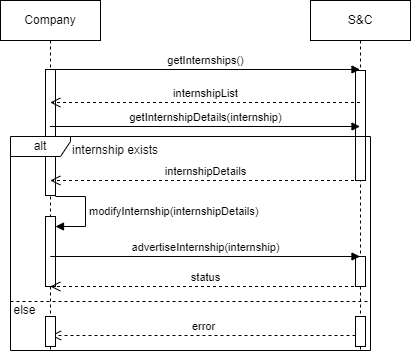
\includegraphics[scale = 0.7]{sequence_diagrams/SequenceDiagramModifyInternship_v_1_1.png}
            \caption{Log-in}
            \label{fig:modify_internship_sequence_diagram}
        \end{figure}

    \newpage
        
    \textbf{[UC7] - Delete internship}
        \begin{figure}[H]
            \centering
            
\includegraphics[scale = 0.7]{sequence_diagrams/SequenceDiagramDeleteInternship_v_1_0.png}
            \caption{Log-in}
            \label{fig:delete_internship_sequence_diagram}
        \end{figure}

    \newpage
        
    \textbf{[UC8] - Search internship}
        \begin{figure}[H]
            \centering
            
\includegraphics[scale = 0.7]{sequence_diagrams/SequenceDiagramSearchInternship_v_1_0.png}
            \caption{Log-in}
            \label{fig:search_internship_sequence_diagram}
        \end{figure}

    \newpage
        
    \textbf{[UC9] - Recommendation process}
        \begin{figure}[H]
            \centering
            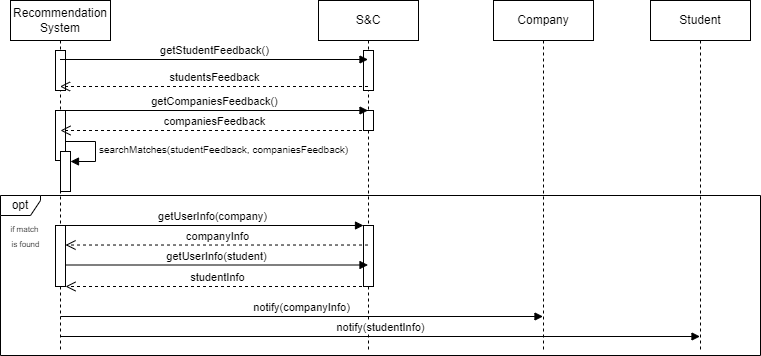
\includegraphics[scale = 0.6]{sequence_diagrams/SequenceDiagramRecommendationProcess_v_1_0.png}
            \caption{Log-in}
            \label{fig:recommendation_process_sequence_diagram}
        \end{figure}

    \newpage
        
    \textbf{[UC10] - Submit application}
        \begin{figure}[H]
            \centering
            
\includegraphics[scale = 0.7]{sequence_diagrams/SequenceDiagramSubmitApplication_v_1_0.png}
            \caption{Log-in}
            \label{fig:submit_application_sequence_diagram}
        \end{figure}

    \newpage
        
    \textbf{[UC11] - Assess application}
        \begin{figure}[H]
            \centering
            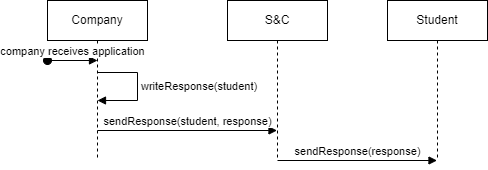
\includegraphics[scale = 0.7]{sequence_diagrams/SequenceAssessApplication_v_1_0.png}
            \caption{Log-in}
            \label{fig:assess_application_sequence_diagram}
        \end{figure}

    \newpage
        
    \textbf{[UC12] - Collect feedback}
        \begin{figure}[H]
            \centering
            
\includegraphics[scale = 0.7]{sequence_diagrams/SequenceDiagramCollectFeedback_v_1_0.png}
            \caption{Log-in}
            \label{fig:collect_feedback_sequence_diagram}
        \end{figure}

    \newpage
        
    \textbf{[UC13] - Selection process}
        \begin{figure}[H]
            \hspace*{-1.5cm}
            \centering
            
\includegraphics[scale = 0.7]{sequence_diagrams/SequenceDiagramSelectionProcess_v_1_0.png}
            \caption{Log-in}
            \label{fig:selection_process_sequence_diagram}
        \end{figure}
        
        \begin{center}
            \begin{longtable}{|l|p{0.75\linewidth}|}
                \hline
                \textbf{Name} & Selection process \\
                \hline
                \textbf{Actors} 
                & Company \\
                & Student \\
                \hline
                \textbf{Entry Condition}
                & Company has sent the student a positive response to their application. \\
                \hline
                \textbf{Event Flow}
                & 1 - Company starts the selection process and notifies student. \\
                & 2 - Company sends the student a questionnaire with the interview questions. \\
                & 3 - Student answers the questions and sends back the compiled questionnaire. \\
                & 4 - Company reads the response and decide wether the candidate is suited or not. \\
                & 5 - If the student is not suited return to step 2. \\
                \hline
                \textbf{Exit Condition}
                & If student is suited the student is hired and the selection process is closed. Otherwise the process is interrupted and the student is notified. \\
                \hline
                \textbf{Exception}
                & Student does not answer the questionnaires. \\
                \hline
            \end{longtable}
        \end{center}

\subsubsection{Requirement Mapping}

\subsection{Performance Requirements}

\subsection{Design Constraint}

\subsubsection{Standard compliance}

\subsubsection{Hardware limitations}

\subsubsection{Any other constraint}

\subsection{Software System Attributes}

\subsubsection{Reliability}

\subsubsection{Availability}

\subsubsection{Security}

\subsubsection{Maintainability}

\subsubsection{Portability}

\section{Alloy} %Mettere titolo giusto
    \begin{comment}
        SEGNARSI IDEE PER ALLOY:
    \end{comment}

\end{document}
